% Options for packages loaded elsewhere
% Options for packages loaded elsewhere
\PassOptionsToPackage{unicode}{hyperref}
\PassOptionsToPackage{hyphens}{url}
\PassOptionsToPackage{dvipsnames,svgnames,x11names}{xcolor}
%
\documentclass[
  letterpaper,
  DIV=11,
  numbers=noendperiod]{scrartcl}
\usepackage{xcolor}
\usepackage{amsmath,amssymb}
\setcounter{secnumdepth}{-\maxdimen} % remove section numbering
\usepackage{iftex}
\ifPDFTeX
  \usepackage[T1]{fontenc}
  \usepackage[utf8]{inputenc}
  \usepackage{textcomp} % provide euro and other symbols
\else % if luatex or xetex
  \usepackage{unicode-math} % this also loads fontspec
  \defaultfontfeatures{Scale=MatchLowercase}
  \defaultfontfeatures[\rmfamily]{Ligatures=TeX,Scale=1}
\fi
\usepackage{lmodern}
\ifPDFTeX\else
  % xetex/luatex font selection
\fi
% Use upquote if available, for straight quotes in verbatim environments
\IfFileExists{upquote.sty}{\usepackage{upquote}}{}
\IfFileExists{microtype.sty}{% use microtype if available
  \usepackage[]{microtype}
  \UseMicrotypeSet[protrusion]{basicmath} % disable protrusion for tt fonts
}{}
\makeatletter
\@ifundefined{KOMAClassName}{% if non-KOMA class
  \IfFileExists{parskip.sty}{%
    \usepackage{parskip}
  }{% else
    \setlength{\parindent}{0pt}
    \setlength{\parskip}{6pt plus 2pt minus 1pt}}
}{% if KOMA class
  \KOMAoptions{parskip=half}}
\makeatother
% Make \paragraph and \subparagraph free-standing
\makeatletter
\ifx\paragraph\undefined\else
  \let\oldparagraph\paragraph
  \renewcommand{\paragraph}{
    \@ifstar
      \xxxParagraphStar
      \xxxParagraphNoStar
  }
  \newcommand{\xxxParagraphStar}[1]{\oldparagraph*{#1}\mbox{}}
  \newcommand{\xxxParagraphNoStar}[1]{\oldparagraph{#1}\mbox{}}
\fi
\ifx\subparagraph\undefined\else
  \let\oldsubparagraph\subparagraph
  \renewcommand{\subparagraph}{
    \@ifstar
      \xxxSubParagraphStar
      \xxxSubParagraphNoStar
  }
  \newcommand{\xxxSubParagraphStar}[1]{\oldsubparagraph*{#1}\mbox{}}
  \newcommand{\xxxSubParagraphNoStar}[1]{\oldsubparagraph{#1}\mbox{}}
\fi
\makeatother

\usepackage{color}
\usepackage{fancyvrb}
\newcommand{\VerbBar}{|}
\newcommand{\VERB}{\Verb[commandchars=\\\{\}]}
\DefineVerbatimEnvironment{Highlighting}{Verbatim}{commandchars=\\\{\}}
% Add ',fontsize=\small' for more characters per line
\usepackage{framed}
\definecolor{shadecolor}{RGB}{241,243,245}
\newenvironment{Shaded}{\begin{snugshade}}{\end{snugshade}}
\newcommand{\AlertTok}[1]{\textcolor[rgb]{0.68,0.00,0.00}{#1}}
\newcommand{\AnnotationTok}[1]{\textcolor[rgb]{0.37,0.37,0.37}{#1}}
\newcommand{\AttributeTok}[1]{\textcolor[rgb]{0.40,0.45,0.13}{#1}}
\newcommand{\BaseNTok}[1]{\textcolor[rgb]{0.68,0.00,0.00}{#1}}
\newcommand{\BuiltInTok}[1]{\textcolor[rgb]{0.00,0.23,0.31}{#1}}
\newcommand{\CharTok}[1]{\textcolor[rgb]{0.13,0.47,0.30}{#1}}
\newcommand{\CommentTok}[1]{\textcolor[rgb]{0.37,0.37,0.37}{#1}}
\newcommand{\CommentVarTok}[1]{\textcolor[rgb]{0.37,0.37,0.37}{\textit{#1}}}
\newcommand{\ConstantTok}[1]{\textcolor[rgb]{0.56,0.35,0.01}{#1}}
\newcommand{\ControlFlowTok}[1]{\textcolor[rgb]{0.00,0.23,0.31}{\textbf{#1}}}
\newcommand{\DataTypeTok}[1]{\textcolor[rgb]{0.68,0.00,0.00}{#1}}
\newcommand{\DecValTok}[1]{\textcolor[rgb]{0.68,0.00,0.00}{#1}}
\newcommand{\DocumentationTok}[1]{\textcolor[rgb]{0.37,0.37,0.37}{\textit{#1}}}
\newcommand{\ErrorTok}[1]{\textcolor[rgb]{0.68,0.00,0.00}{#1}}
\newcommand{\ExtensionTok}[1]{\textcolor[rgb]{0.00,0.23,0.31}{#1}}
\newcommand{\FloatTok}[1]{\textcolor[rgb]{0.68,0.00,0.00}{#1}}
\newcommand{\FunctionTok}[1]{\textcolor[rgb]{0.28,0.35,0.67}{#1}}
\newcommand{\ImportTok}[1]{\textcolor[rgb]{0.00,0.46,0.62}{#1}}
\newcommand{\InformationTok}[1]{\textcolor[rgb]{0.37,0.37,0.37}{#1}}
\newcommand{\KeywordTok}[1]{\textcolor[rgb]{0.00,0.23,0.31}{\textbf{#1}}}
\newcommand{\NormalTok}[1]{\textcolor[rgb]{0.00,0.23,0.31}{#1}}
\newcommand{\OperatorTok}[1]{\textcolor[rgb]{0.37,0.37,0.37}{#1}}
\newcommand{\OtherTok}[1]{\textcolor[rgb]{0.00,0.23,0.31}{#1}}
\newcommand{\PreprocessorTok}[1]{\textcolor[rgb]{0.68,0.00,0.00}{#1}}
\newcommand{\RegionMarkerTok}[1]{\textcolor[rgb]{0.00,0.23,0.31}{#1}}
\newcommand{\SpecialCharTok}[1]{\textcolor[rgb]{0.37,0.37,0.37}{#1}}
\newcommand{\SpecialStringTok}[1]{\textcolor[rgb]{0.13,0.47,0.30}{#1}}
\newcommand{\StringTok}[1]{\textcolor[rgb]{0.13,0.47,0.30}{#1}}
\newcommand{\VariableTok}[1]{\textcolor[rgb]{0.07,0.07,0.07}{#1}}
\newcommand{\VerbatimStringTok}[1]{\textcolor[rgb]{0.13,0.47,0.30}{#1}}
\newcommand{\WarningTok}[1]{\textcolor[rgb]{0.37,0.37,0.37}{\textit{#1}}}

\usepackage{longtable,booktabs,array}
\usepackage{calc} % for calculating minipage widths
% Correct order of tables after \paragraph or \subparagraph
\usepackage{etoolbox}
\makeatletter
\patchcmd\longtable{\par}{\if@noskipsec\mbox{}\fi\par}{}{}
\makeatother
% Allow footnotes in longtable head/foot
\IfFileExists{footnotehyper.sty}{\usepackage{footnotehyper}}{\usepackage{footnote}}
\makesavenoteenv{longtable}
\usepackage{graphicx}
\makeatletter
\newsavebox\pandoc@box
\newcommand*\pandocbounded[1]{% scales image to fit in text height/width
  \sbox\pandoc@box{#1}%
  \Gscale@div\@tempa{\textheight}{\dimexpr\ht\pandoc@box+\dp\pandoc@box\relax}%
  \Gscale@div\@tempb{\linewidth}{\wd\pandoc@box}%
  \ifdim\@tempb\p@<\@tempa\p@\let\@tempa\@tempb\fi% select the smaller of both
  \ifdim\@tempa\p@<\p@\scalebox{\@tempa}{\usebox\pandoc@box}%
  \else\usebox{\pandoc@box}%
  \fi%
}
% Set default figure placement to htbp
\def\fps@figure{htbp}
\makeatother





\setlength{\emergencystretch}{3em} % prevent overfull lines

\providecommand{\tightlist}{%
  \setlength{\itemsep}{0pt}\setlength{\parskip}{0pt}}



 


\KOMAoption{captions}{tableheading}
\makeatletter
\@ifpackageloaded{tcolorbox}{}{\usepackage[skins,breakable]{tcolorbox}}
\@ifpackageloaded{fontawesome5}{}{\usepackage{fontawesome5}}
\definecolor{quarto-callout-color}{HTML}{909090}
\definecolor{quarto-callout-note-color}{HTML}{0758E5}
\definecolor{quarto-callout-important-color}{HTML}{CC1914}
\definecolor{quarto-callout-warning-color}{HTML}{EB9113}
\definecolor{quarto-callout-tip-color}{HTML}{00A047}
\definecolor{quarto-callout-caution-color}{HTML}{FC5300}
\definecolor{quarto-callout-color-frame}{HTML}{acacac}
\definecolor{quarto-callout-note-color-frame}{HTML}{4582ec}
\definecolor{quarto-callout-important-color-frame}{HTML}{d9534f}
\definecolor{quarto-callout-warning-color-frame}{HTML}{f0ad4e}
\definecolor{quarto-callout-tip-color-frame}{HTML}{02b875}
\definecolor{quarto-callout-caution-color-frame}{HTML}{fd7e14}
\makeatother
\makeatletter
\@ifpackageloaded{caption}{}{\usepackage{caption}}
\AtBeginDocument{%
\ifdefined\contentsname
  \renewcommand*\contentsname{Table of contents}
\else
  \newcommand\contentsname{Table of contents}
\fi
\ifdefined\listfigurename
  \renewcommand*\listfigurename{List of Figures}
\else
  \newcommand\listfigurename{List of Figures}
\fi
\ifdefined\listtablename
  \renewcommand*\listtablename{List of Tables}
\else
  \newcommand\listtablename{List of Tables}
\fi
\ifdefined\figurename
  \renewcommand*\figurename{Figure}
\else
  \newcommand\figurename{Figure}
\fi
\ifdefined\tablename
  \renewcommand*\tablename{Table}
\else
  \newcommand\tablename{Table}
\fi
}
\@ifpackageloaded{float}{}{\usepackage{float}}
\floatstyle{ruled}
\@ifundefined{c@chapter}{\newfloat{codelisting}{h}{lop}}{\newfloat{codelisting}{h}{lop}[chapter]}
\floatname{codelisting}{Listing}
\newcommand*\listoflistings{\listof{codelisting}{List of Listings}}
\makeatother
\makeatletter
\makeatother
\makeatletter
\@ifpackageloaded{caption}{}{\usepackage{caption}}
\@ifpackageloaded{subcaption}{}{\usepackage{subcaption}}
\makeatother
\usepackage{bookmark}
\IfFileExists{xurl.sty}{\usepackage{xurl}}{} % add URL line breaks if available
\urlstyle{same}
\hypersetup{
  pdftitle={Decision Tree Challenge},
  colorlinks=true,
  linkcolor={blue},
  filecolor={Maroon},
  citecolor={Blue},
  urlcolor={Blue},
  pdfcreator={LaTeX via pandoc}}


\title{Decision Tree Challenge}
\usepackage{etoolbox}
\makeatletter
\providecommand{\subtitle}[1]{% add subtitle to \maketitle
  \apptocmd{\@title}{\par {\large #1 \par}}{}{}
}
\makeatother
\subtitle{Feature Importance and Categorical Variable Encoding}
\author{}
\date{}
\begin{document}
\maketitle


\section{🌳 Decision Tree Challenge - Feature Importance and Variable
Encoding}\label{decision-tree-challenge---feature-importance-and-variable-encoding}

\hyperref[discussion-questions-for-challenge]{📋 Jump to Discussion
Questions}

\subsection{Challenge Overview}\label{challenge-overview}

\textbf{Your Mission:} Create a simple GitHub Pages site that
demonstrates how decision trees measure feature importance and analyzes
the critical differences between categorical and numerical variable
encoding. You'll answer two key discussion questions by adding narrative
to a pre-built analysis and posting those answers to your GitHub Pages
site as a rendered HTML document.

\begin{tcolorbox}[enhanced jigsaw, colbacktitle=quarto-callout-warning-color!10!white, toptitle=1mm, colframe=quarto-callout-warning-color-frame, breakable, rightrule=.15mm, arc=.35mm, bottomtitle=1mm, titlerule=0mm, opacityback=0, title=\textcolor{quarto-callout-warning-color}{\faExclamationTriangle}\hspace{0.5em}{⚠️ AI Partnership Required}, colback=white, bottomrule=.15mm, toprule=.15mm, leftrule=.75mm, coltitle=black, opacitybacktitle=0.6, left=2mm]

This challenge pushes boundaries intentionally. You'll tackle problems
that normally require weeks of study, but with Cursor AI as your partner
(and your brain keeping it honest), you can accomplish more than you
thought possible.

\textbf{The new reality:} The four stages of competence are Ignorance →
Awareness → Learning → Mastery. AI lets us produce Mastery-level work
while operating primarily in the Awareness stage. I focus on awareness
training, you leverage AI for execution, and together we create outputs
that used to require years of dedicated study.

\end{tcolorbox}

\subsection{The Decision Tree Problem
🎯}\label{the-decision-tree-problem}

\begin{quote}
``The most important thing in communication is hearing what isn't
said.'' - Peter Drucker
\end{quote}

\textbf{The Core Problem:} Decision trees are often praised for their
interpretability and ability to handle both numerical and categorical
variables. But what happens when we encode categorical variables as
numbers? How does this affect our understanding of feature importance?

\textbf{What is Feature Importance?} In decision trees, feature
importance measures how much each variable contributes to reducing
impurity (or improving prediction accuracy) across all splits in the
tree. It's a key metric for understanding which variables matter most
for your predictions.

\begin{tcolorbox}[enhanced jigsaw, colbacktitle=quarto-callout-important-color!10!white, toptitle=1mm, colframe=quarto-callout-important-color-frame, breakable, rightrule=.15mm, arc=.35mm, bottomtitle=1mm, titlerule=0mm, opacityback=0, title=\textcolor{quarto-callout-important-color}{\faExclamation}\hspace{0.5em}{🎯 The Key Insight: Encoding Matters for Interpretability}, colback=white, bottomrule=.15mm, toprule=.15mm, leftrule=.75mm, coltitle=black, opacitybacktitle=0.6, left=2mm]

\textbf{The problem:} When we encode categorical variables as numerical
values (like 1, 2, 3, 4\ldots), decision trees treat them as if they
have a meaningful numerical order. This can completely distort our
analysis.

\textbf{The Real-World Context:} In real estate, we know that
neighborhood quality, house style, and other categorical factors are
crucial for predicting home prices. But if we encode these as numbers,
we might get misleading insights about which features actually matter
most.

\textbf{The Devastating Reality:} Even sophisticated machine learning
models can give us completely wrong insights about feature importance if
we don't properly encode our variables. A categorical variable that
should be among the most important might appear irrelevant, while a
numerical variable might appear artificially important.

\end{tcolorbox}

Let's assume we want to predict house prices and understand which
features matter most. The key question is: \textbf{How does encoding
categorical variables as numbers affect our understanding of feature
importance?}

\subsection{The Ames Housing Dataset 🏠}\label{the-ames-housing-dataset}

We are analyzing the Ames Housing dataset which contains detailed
information about residential properties sold in Ames, Iowa from 2006 to
2010. This dataset is perfect for our analysis because it contains a
categorical variable (like zip code) and numerical variables (like
square footage, year built, number of bedrooms).

\subsection{The Problem: ZipCode as Numerical vs
Categorical}\label{the-problem-zipcode-as-numerical-vs-categorical}

\textbf{Key Question:} What happens when we treat zipCode as a numerical
variable in a decision tree? How does this affect feature importance
interpretation?

\textbf{The Issue:} Zip codes (50010, 50011, 50012, 50013) are
categorical variables representing discrete geographic areas,
i.e.~neighborhoods. When treated as numerical, the tree might split on
``zipCode \textgreater{} 50012.5'' - which has no meaningful
interpretation for house prices. Zip codes are non-ordinal categorical
variables meaning they have no inherent order that aids house price
prediction (i.e.~zip code 99999 is not the priceiest zip code).

\subsection{Data Loading and Model
Building}\label{data-loading-and-model-building}

\begin{Shaded}
\begin{Highlighting}[]
\CommentTok{\# Load libraries}
\FunctionTok{suppressPackageStartupMessages}\NormalTok{(}\FunctionTok{library}\NormalTok{(tidyverse))}
\FunctionTok{suppressPackageStartupMessages}\NormalTok{(}\FunctionTok{library}\NormalTok{(rpart))}
\ControlFlowTok{if}\NormalTok{ (}\SpecialCharTok{!}\FunctionTok{require}\NormalTok{(rpart.plot, }\AttributeTok{quietly =} \ConstantTok{TRUE}\NormalTok{)) \{}
  \FunctionTok{install.packages}\NormalTok{(}\StringTok{"rpart.plot"}\NormalTok{, }\AttributeTok{repos =} \StringTok{"https://cran.rstudio.com/"}\NormalTok{)}
  \FunctionTok{library}\NormalTok{(rpart.plot)}
\NormalTok{\}}

\CommentTok{\# Load data}
\NormalTok{sales\_data }\OtherTok{\textless{}{-}} \FunctionTok{read.csv}\NormalTok{(}\StringTok{"https://raw.githubusercontent.com/flyaflya/buad442Fall2025/refs/heads/main/datasets/salesPriceData.csv"}\NormalTok{)}

\CommentTok{\# Prepare model data (treating zipCode as numerical)}
\NormalTok{model\_data }\OtherTok{\textless{}{-}}\NormalTok{ sales\_data }\SpecialCharTok{\%\textgreater{}\%}
  \FunctionTok{select}\NormalTok{(SalePrice, LotArea, YearBuilt, GrLivArea, FullBath, HalfBath, }
\NormalTok{         BedroomAbvGr, TotRmsAbvGrd, GarageCars, zipCode) }\SpecialCharTok{\%\textgreater{}\%}
  \FunctionTok{na.omit}\NormalTok{()}

\CommentTok{\# Split data}
\FunctionTok{set.seed}\NormalTok{(}\DecValTok{123}\NormalTok{)}
\NormalTok{train\_indices }\OtherTok{\textless{}{-}} \FunctionTok{sample}\NormalTok{(}\DecValTok{1}\SpecialCharTok{:}\FunctionTok{nrow}\NormalTok{(model\_data), }\FloatTok{0.8} \SpecialCharTok{*} \FunctionTok{nrow}\NormalTok{(model\_data))}
\NormalTok{train\_data }\OtherTok{\textless{}{-}}\NormalTok{ model\_data[train\_indices, ]}
\NormalTok{test\_data }\OtherTok{\textless{}{-}}\NormalTok{ model\_data[}\SpecialCharTok{{-}}\NormalTok{train\_indices, ]}

\CommentTok{\# Build decision tree}
\NormalTok{tree\_model }\OtherTok{\textless{}{-}} \FunctionTok{rpart}\NormalTok{(SalePrice }\SpecialCharTok{\textasciitilde{}}\NormalTok{ ., }
                    \AttributeTok{data =}\NormalTok{ train\_data,}
                    \AttributeTok{method =} \StringTok{"anova"}\NormalTok{,}
                    \AttributeTok{control =} \FunctionTok{rpart.control}\NormalTok{(}\AttributeTok{maxdepth =} \DecValTok{3}\NormalTok{, }
                                          \AttributeTok{minsplit =} \DecValTok{20}\NormalTok{, }
                                          \AttributeTok{minbucket =} \DecValTok{10}\NormalTok{))}

\FunctionTok{cat}\NormalTok{(}\StringTok{"Model built with"}\NormalTok{, }\FunctionTok{sum}\NormalTok{(tree\_model}\SpecialCharTok{$}\NormalTok{frame}\SpecialCharTok{$}\NormalTok{var }\SpecialCharTok{==} \StringTok{"\textless{}leaf\textgreater{}"}\NormalTok{), }\StringTok{"terminal nodes}\SpecialCharTok{\textbackslash{}n}\StringTok{"}\NormalTok{)}
\end{Highlighting}
\end{Shaded}

\begin{verbatim}
Model built with 7 terminal nodes
\end{verbatim}

\subsection{Tree Visualization}\label{tree-visualization}

\begin{Shaded}
\begin{Highlighting}[]
\CommentTok{\# Visualize tree}
\ControlFlowTok{if}\NormalTok{ (}\FunctionTok{require}\NormalTok{(rpart.plot, }\AttributeTok{quietly =} \ConstantTok{TRUE}\NormalTok{)) \{}
  \FunctionTok{rpart.plot}\NormalTok{(tree\_model, }
             \AttributeTok{type =} \DecValTok{2}\NormalTok{,}
             \AttributeTok{extra =} \DecValTok{101}\NormalTok{,}
             \AttributeTok{fallen.leaves =} \ConstantTok{TRUE}\NormalTok{,}
             \AttributeTok{digits =} \DecValTok{0}\NormalTok{,}
             \AttributeTok{cex =} \FloatTok{0.8}\NormalTok{,}
             \AttributeTok{main =} \StringTok{"Decision Tree (zipCode as Numerical)"}\NormalTok{)}
\NormalTok{\} }\ControlFlowTok{else}\NormalTok{ \{}
  \FunctionTok{plot}\NormalTok{(tree\_model, }\AttributeTok{uniform =} \ConstantTok{TRUE}\NormalTok{, }\AttributeTok{main =} \StringTok{"Decision Tree (zipCode as Numerical)"}\NormalTok{)}
  \FunctionTok{text}\NormalTok{(tree\_model, }\AttributeTok{use.n =} \ConstantTok{TRUE}\NormalTok{, }\AttributeTok{all =} \ConstantTok{TRUE}\NormalTok{, }\AttributeTok{cex =} \FloatTok{0.8}\NormalTok{)}
\NormalTok{\}}
\end{Highlighting}
\end{Shaded}

\pandocbounded{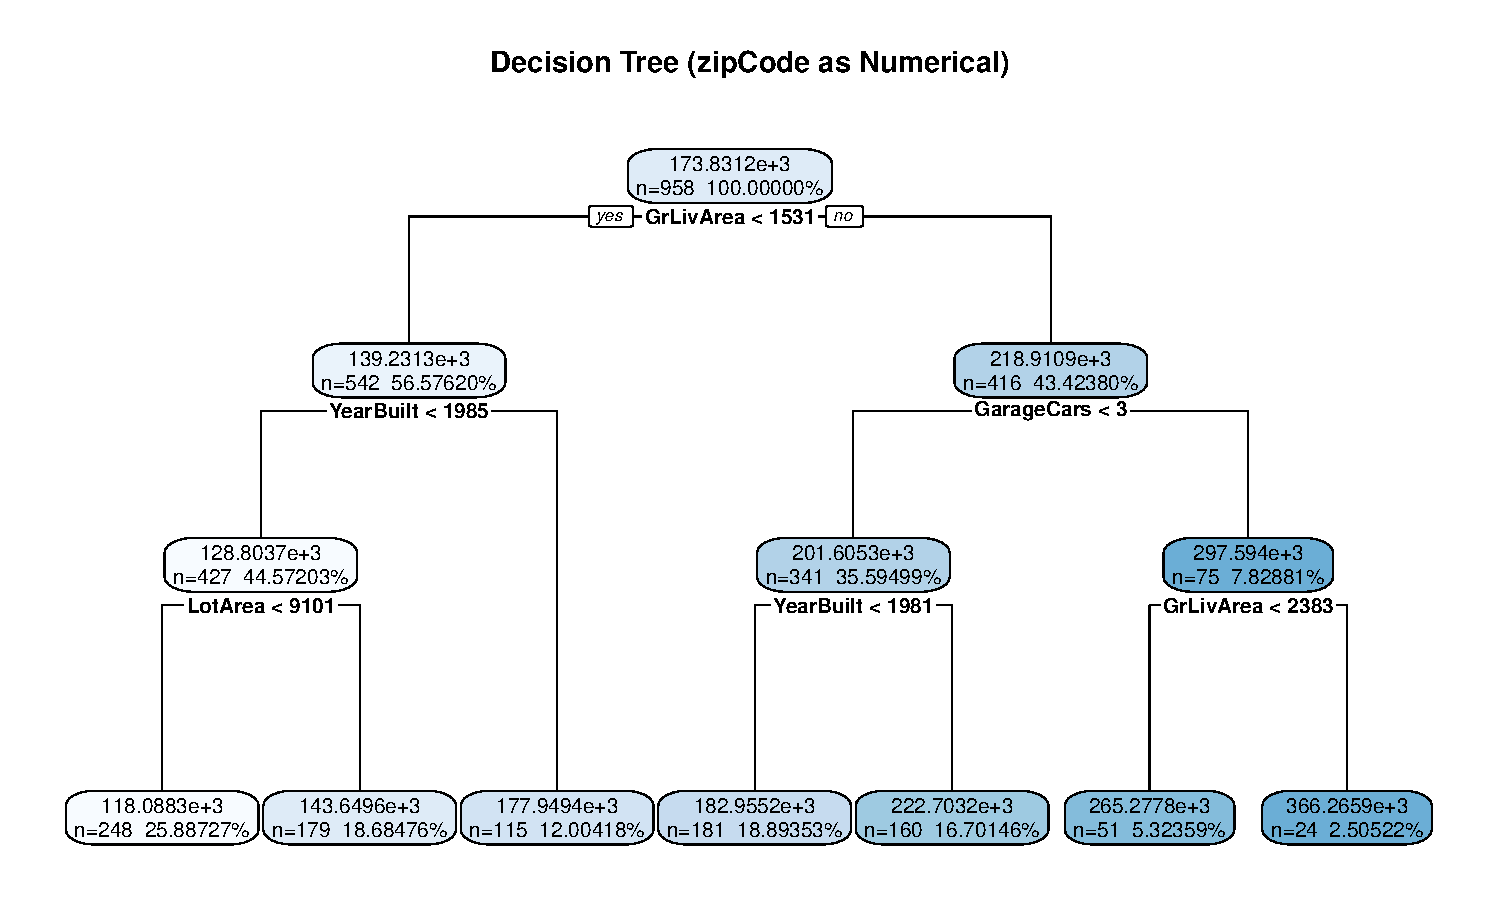
\includegraphics[keepaspectratio]{index_files/figure-pdf/visualize-tree-r-1.pdf}}

\subsection{Feature Importance
Analysis}\label{feature-importance-analysis}

\pandocbounded{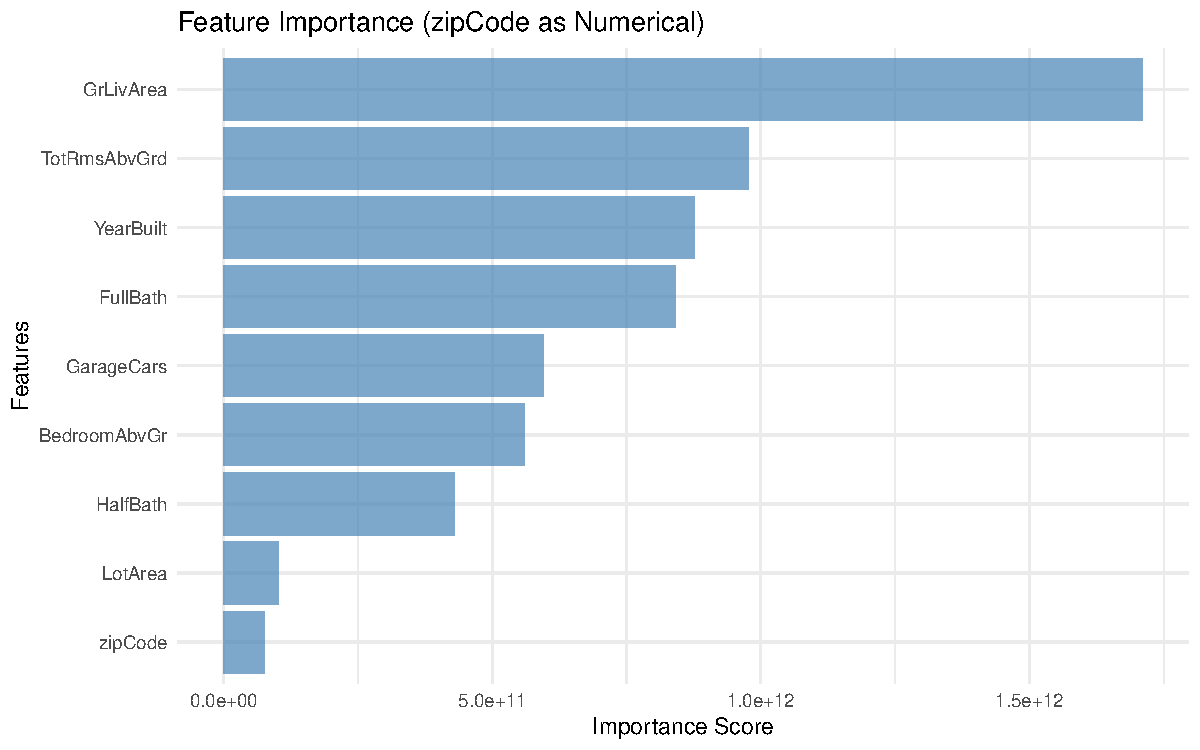
\includegraphics[keepaspectratio]{index_files/figure-pdf/importance-plot-r-1.pdf}}

:::

\subsection{Critical Analysis: The Encoding
Problem}\label{critical-analysis-the-encoding-problem}

\begin{tcolorbox}[enhanced jigsaw, colbacktitle=quarto-callout-warning-color!10!white, toptitle=1mm, colframe=quarto-callout-warning-color-frame, breakable, rightrule=.15mm, arc=.35mm, bottomtitle=1mm, titlerule=0mm, opacityback=0, title=\textcolor{quarto-callout-warning-color}{\faExclamationTriangle}\hspace{0.5em}{⚠️ The Problem Revealed}, colback=white, bottomrule=.15mm, toprule=.15mm, leftrule=.75mm, coltitle=black, opacitybacktitle=0.6, left=2mm]

\textbf{What to note:} Our decision tree treated \texttt{zipCode} as a
numerical variable. This leads to zip code being unimportant. Not
surprisingly, because there is no reason to believe allowing splits like
``zipCode \textless{} 50012.5'' should be beneficial for house price
prediction. This false coding of a variable creates several problems:

\begin{enumerate}
\def\labelenumi{\arabic{enumi}.}
\tightlist
\item
  \textbf{Potentially Meaningless Splits:} A zip code of 50013 is not
  ``greater than'' 50012 in any meaningful way for house prices
\item
  \textbf{False Importance:} The algorithm assigns importance to zipCode
  based on numerical splits rather than categorical distinctions OR the
  importance of zip code is completely missed as numerical ordering has
  no inherent relationship to house prices.
\item
  \textbf{Misleading Interpretations:} We might conclude zipCode is not
  important when our intuition tells us it should be important (listen
  to your intuition).
\end{enumerate}

\textbf{The Real Issue:} Zip codes are categorical variables
representing discrete geographic areas. The numerical values have no
inherent order or magnitude relationship to house prices. These must be
modelled as categorical variables.

\end{tcolorbox}

\subsection{Proper Categorical Encoding: The
Solution}\label{proper-categorical-encoding-the-solution}

Now let's repeat the analysis with zipCode properly encoded as
categorical variables to see the difference.

\textbf{R Approach:} Convert zipCode to a factor (categorical
variable)\\
\textbf{Python Approach:} One-hot encode zipCode (create dummy variables
for each zip code)

\subsubsection{Categorical Encoding
Analysis}\label{categorical-encoding-analysis}

\begin{Shaded}
\begin{Highlighting}[]
\CommentTok{\# Convert zipCode to factor (categorical)}
\NormalTok{model\_data\_cat }\OtherTok{\textless{}{-}}\NormalTok{ model\_data }\SpecialCharTok{\%\textgreater{}\%}
  \FunctionTok{mutate}\NormalTok{(}\AttributeTok{zipCode =} \FunctionTok{as.factor}\NormalTok{(zipCode))}

\CommentTok{\# Split data}
\FunctionTok{set.seed}\NormalTok{(}\DecValTok{123}\NormalTok{)}
\NormalTok{train\_indices\_cat }\OtherTok{\textless{}{-}} \FunctionTok{sample}\NormalTok{(}\DecValTok{1}\SpecialCharTok{:}\FunctionTok{nrow}\NormalTok{(model\_data\_cat), }\FloatTok{0.8} \SpecialCharTok{*} \FunctionTok{nrow}\NormalTok{(model\_data\_cat))}
\NormalTok{train\_data\_cat }\OtherTok{\textless{}{-}}\NormalTok{ model\_data\_cat[train\_indices\_cat, ]}
\NormalTok{test\_data\_cat }\OtherTok{\textless{}{-}}\NormalTok{ model\_data\_cat[}\SpecialCharTok{{-}}\NormalTok{train\_indices\_cat, ]}

\CommentTok{\# Build decision tree with categorical zipCode}
\NormalTok{tree\_model\_cat }\OtherTok{\textless{}{-}} \FunctionTok{rpart}\NormalTok{(SalePrice }\SpecialCharTok{\textasciitilde{}}\NormalTok{ ., }
                        \AttributeTok{data =}\NormalTok{ train\_data\_cat,}
                        \AttributeTok{method =} \StringTok{"anova"}\NormalTok{,}
                        \AttributeTok{control =} \FunctionTok{rpart.control}\NormalTok{(}\AttributeTok{maxdepth =} \DecValTok{3}\NormalTok{, }
                                              \AttributeTok{minsplit =} \DecValTok{20}\NormalTok{, }
                                              \AttributeTok{minbucket =} \DecValTok{10}\NormalTok{))}

\CommentTok{\# Feature importance with categorical zipCode}
\NormalTok{importance\_cat }\OtherTok{\textless{}{-}} \FunctionTok{data.frame}\NormalTok{(}
  \AttributeTok{Feature =} \FunctionTok{names}\NormalTok{(tree\_model\_cat}\SpecialCharTok{$}\NormalTok{variable.importance),}
  \AttributeTok{Importance =} \FunctionTok{as.numeric}\NormalTok{(tree\_model\_cat}\SpecialCharTok{$}\NormalTok{variable.importance)}
\NormalTok{) }\SpecialCharTok{\%\textgreater{}\%}
  \FunctionTok{arrange}\NormalTok{(}\FunctionTok{desc}\NormalTok{(Importance)) }\SpecialCharTok{\%\textgreater{}\%}
  \FunctionTok{mutate}\NormalTok{(}\AttributeTok{Importance\_Percent =} \FunctionTok{round}\NormalTok{(Importance }\SpecialCharTok{/} \FunctionTok{sum}\NormalTok{(Importance) }\SpecialCharTok{*} \DecValTok{100}\NormalTok{, }\DecValTok{2}\NormalTok{))}

\CommentTok{\# Check if zipCode appears in tree}
\NormalTok{zipcode\_in\_tree }\OtherTok{\textless{}{-}} \StringTok{"zipCode"} \SpecialCharTok{\%in\%} \FunctionTok{names}\NormalTok{(tree\_model\_cat}\SpecialCharTok{$}\NormalTok{variable.importance)}
\ControlFlowTok{if}\NormalTok{(zipcode\_in\_tree) \{}
\NormalTok{  zipcode\_rank\_cat }\OtherTok{\textless{}{-}} \FunctionTok{which}\NormalTok{(importance\_cat}\SpecialCharTok{$}\NormalTok{Feature }\SpecialCharTok{==} \StringTok{"zipCode"}\NormalTok{)}
\NormalTok{\}}
\end{Highlighting}
\end{Shaded}

\subsubsection{Tree Visualization: Categorical
zipCode}\label{tree-visualization-categorical-zipcode}

\begin{Shaded}
\begin{Highlighting}[]
\CommentTok{\# Visualize tree with categorical zipCode}
\ControlFlowTok{if}\NormalTok{ (}\FunctionTok{require}\NormalTok{(rpart.plot, }\AttributeTok{quietly =} \ConstantTok{TRUE}\NormalTok{)) \{}
  \FunctionTok{rpart.plot}\NormalTok{(tree\_model\_cat, }
             \AttributeTok{type =} \DecValTok{2}\NormalTok{,}
             \AttributeTok{extra =} \DecValTok{101}\NormalTok{,}
             \AttributeTok{fallen.leaves =} \ConstantTok{TRUE}\NormalTok{,}
             \AttributeTok{digits =} \DecValTok{0}\NormalTok{,}
             \AttributeTok{cex =} \FloatTok{0.8}\NormalTok{,}
             \AttributeTok{main =} \StringTok{"Decision Tree (zipCode as Categorical)"}\NormalTok{)}
\NormalTok{\} }\ControlFlowTok{else}\NormalTok{ \{}
  \FunctionTok{plot}\NormalTok{(tree\_model\_cat, }\AttributeTok{uniform =} \ConstantTok{TRUE}\NormalTok{, }\AttributeTok{main =} \StringTok{"Decision Tree (zipCode as Categorical)"}\NormalTok{)}
  \FunctionTok{text}\NormalTok{(tree\_model\_cat, }\AttributeTok{use.n =} \ConstantTok{TRUE}\NormalTok{, }\AttributeTok{all =} \ConstantTok{TRUE}\NormalTok{, }\AttributeTok{cex =} \FloatTok{0.8}\NormalTok{)}
\NormalTok{\}}
\end{Highlighting}
\end{Shaded}

\pandocbounded{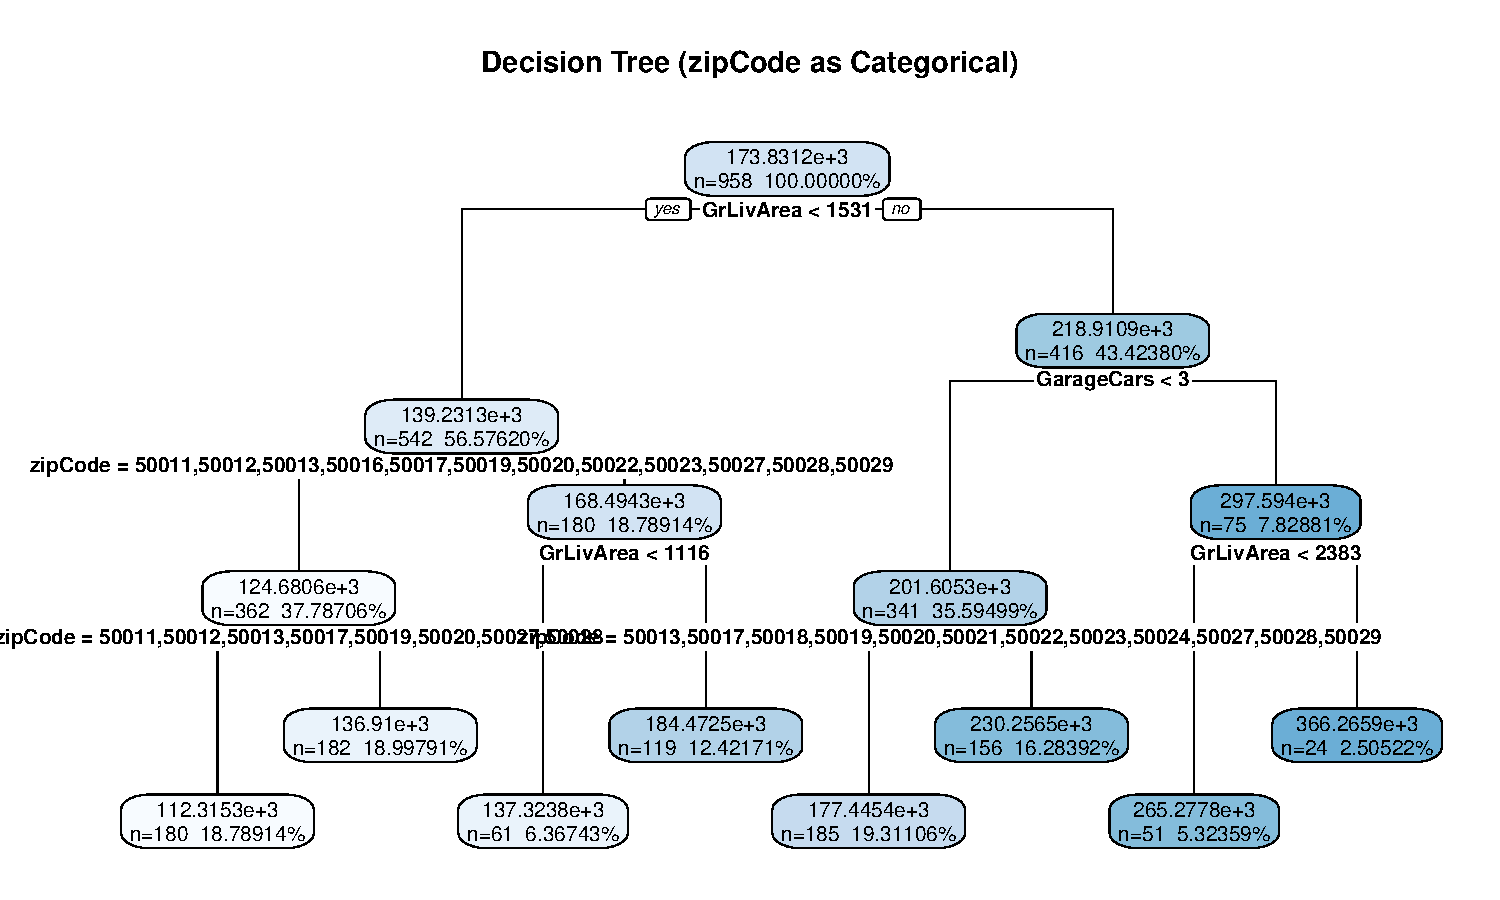
\includegraphics[keepaspectratio]{index_files/figure-pdf/visualize-tree-cat-r-1.pdf}}

\subsubsection{Feature Importance: Categorical
zipCode}\label{feature-importance-categorical-zipcode}

\pandocbounded{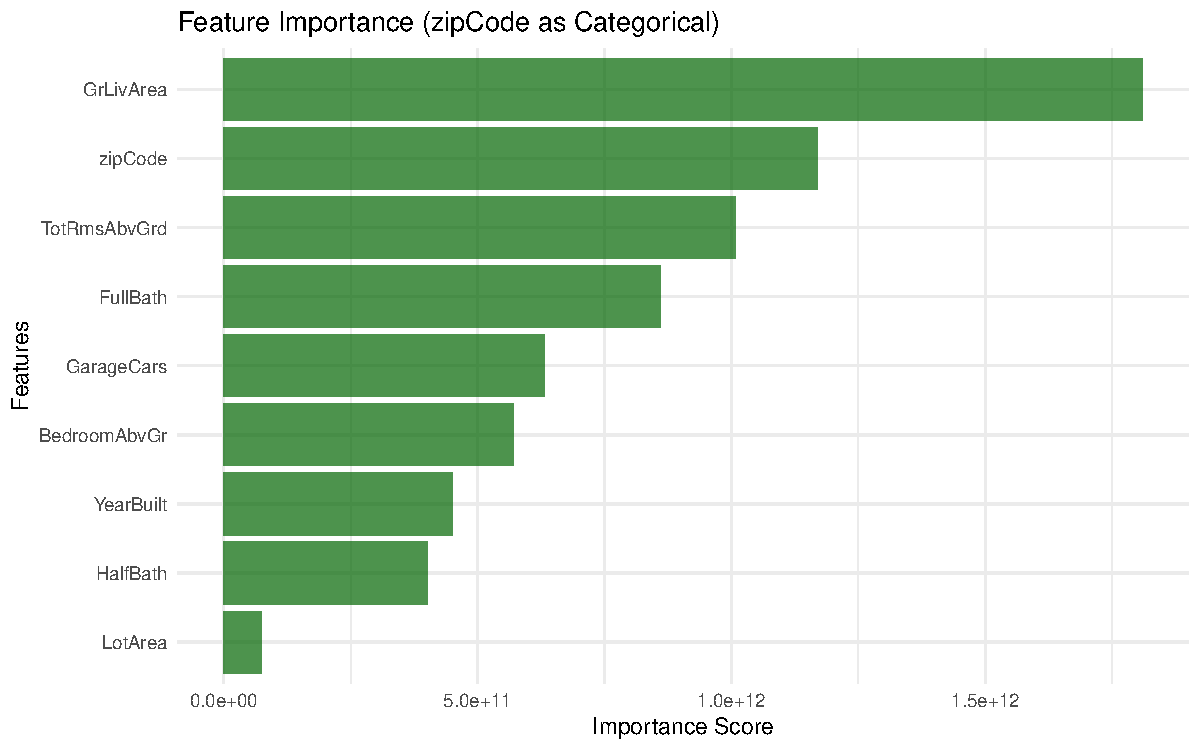
\includegraphics[keepaspectratio]{index_files/figure-pdf/importance-plot-cat-r-1.pdf}}

\subsection{Challenge Requirements 📋}\label{challenge-requirements}

\subsubsection{Minimum Requirements for Any Points on
Challenge}\label{minimum-requirements-for-any-points-on-challenge}

\begin{enumerate}
\def\labelenumi{\arabic{enumi}.}
\item
  \textbf{Create a GitHub Pages Site:} Use the starter repository (see
  Repository Setup section below) to begin with a working template. The
  repository includes all the analysis code and visualizations above.
\item
  \textbf{Add Discussion Narrative:} Add your answers to the two
  discussion questions below in the Discussion Questions section of the
  rendered HTML.
\item
  \textbf{GitHub Repository:} Use your forked repository (from the
  starter repository) named ``decTreeChallenge'' in your GitHub account.
\item
  \textbf{GitHub Pages Setup:} The repository should be made the source
  of your github pages:

  \begin{itemize}
  \tightlist
  \item
    Go to your repository settings (click the ``Settings'' tab in your
    GitHub repository)
  \item
    Scroll down to the ``Pages'' section in the left sidebar
  \item
    Under ``Source'', select ``Deploy from a branch''
  \item
    Choose ``main'' branch and ``/ (root)'' folder
  \item
    Click ``Save''
  \item
    Your site will be available at:
    \texttt{https://{[}your-username{]}.github.io/decTreeChallenge/}
  \item
    \textbf{Note:} It may take a few minutes for the site to become
    available after enabling Pages
  \end{itemize}
\end{enumerate}

\subsection{Getting Started: Repository Setup
🚀}\label{getting-started-repository-setup}

\begin{tcolorbox}[enhanced jigsaw, colbacktitle=quarto-callout-important-color!10!white, toptitle=1mm, colframe=quarto-callout-important-color-frame, breakable, rightrule=.15mm, arc=.35mm, bottomtitle=1mm, titlerule=0mm, opacityback=0, title=\textcolor{quarto-callout-important-color}{\faExclamation}\hspace{0.5em}{📁 Quick Start with Starter Repository}, colback=white, bottomrule=.15mm, toprule=.15mm, leftrule=.75mm, coltitle=black, opacitybacktitle=0.6, left=2mm]

\textbf{Step 1:} Fork the starter repository to your github account at
\url{https://github.com/flyaflya/decTreeChallenge.git}

\textbf{Step 2:} Clone your fork locally using Cursor (or VS Code)

\textbf{Step 3:} You're ready to start! The repository includes
pre-loaded data and a working template with all the analysis above.

\end{tcolorbox}

\begin{tcolorbox}[enhanced jigsaw, colbacktitle=quarto-callout-tip-color!10!white, toptitle=1mm, colframe=quarto-callout-tip-color-frame, breakable, rightrule=.15mm, arc=.35mm, bottomtitle=1mm, titlerule=0mm, opacityback=0, title=\textcolor{quarto-callout-tip-color}{\faLightbulb}\hspace{0.5em}{💡 Why Use the Starter Repository?}, colback=white, bottomrule=.15mm, toprule=.15mm, leftrule=.75mm, coltitle=black, opacitybacktitle=0.6, left=2mm]

\textbf{Benefits:}

\begin{itemize}
\tightlist
\item
  \textbf{Pre-loaded data:} All required data and analysis code is
  included
\item
  \textbf{Working template:} Basic Quarto structure (\texttt{index.qmd})
  is ready
\item
  \textbf{No setup errors:} Avoid common data loading issues
\item
  \textbf{Focus on analysis:} Spend time on the discussion questions,
  not data preparation
\end{itemize}

\end{tcolorbox}

\subsubsection{Getting Started Tips}\label{getting-started-tips}

\begin{tcolorbox}[enhanced jigsaw, colbacktitle=quarto-callout-note-color!10!white, toptitle=1mm, colframe=quarto-callout-note-color-frame, breakable, rightrule=.15mm, arc=.35mm, bottomtitle=1mm, titlerule=0mm, opacityback=0, title=\textcolor{quarto-callout-note-color}{\faInfo}\hspace{0.5em}{🎯 Navy SEALs Motto}, colback=white, bottomrule=.15mm, toprule=.15mm, leftrule=.75mm, coltitle=black, opacitybacktitle=0.6, left=2mm]

\begin{quote}
``Slow is Smooth and Smooth is Fast''
\end{quote}

\emph{Take your time to understand the decision tree mechanics, plan
your approach carefully, and execute with precision. Rushing through
this challenge will only lead to errors and confusion.}

\end{tcolorbox}

\begin{tcolorbox}[enhanced jigsaw, colbacktitle=quarto-callout-warning-color!10!white, toptitle=1mm, colframe=quarto-callout-warning-color-frame, breakable, rightrule=.15mm, arc=.35mm, bottomtitle=1mm, titlerule=0mm, opacityback=0, title=\textcolor{quarto-callout-warning-color}{\faExclamationTriangle}\hspace{0.5em}{💾 Important: Save Your Work Frequently!}, colback=white, bottomrule=.15mm, toprule=.15mm, leftrule=.75mm, coltitle=black, opacitybacktitle=0.6, left=2mm]

\textbf{Before you start:} Make sure to commit your work often using the
Source Control panel in Cursor (Ctrl+Shift+G or Cmd+Shift+G). This
prevents the AI from overwriting your progress and ensures you don't
lose your work.

\textbf{Commit after each major step:}

\begin{itemize}
\tightlist
\item
  After adding your discussion answers
\item
  After rendering to HTML
\item
  Before asking the AI for help with new code
\end{itemize}

\textbf{How to commit:}

\begin{enumerate}
\def\labelenumi{\arabic{enumi}.}
\tightlist
\item
  Open Source Control panel (Ctrl+Shift+G)
\item
  Stage your changes (+ button)
\item
  Write a descriptive commit message
\item
  Click the checkmark to commit
\end{enumerate}

\emph{Remember: Frequent commits are your safety net!}

\end{tcolorbox}

\subsection{Discussion Questions for
Challenge}\label{discussion-questions-for-challenge}

\textbf{Your Task:} Add thoughtful narrative answers to these two
questions in the Discussion Questions section of your rendered HTML
site.

\begin{enumerate}
\def\labelenumi{\arabic{enumi}.}
\tightlist
\item
  \textbf{Numerical vs Categorical Encoding:} There are four models
  above, two in R and two in Python. For each language, the models
  differ by how zip code is modelled, either as a numerical variable or
  as a categorical variable. Given what you know about zip codes and
  real estate prices, how should zip code be modelled, numerically or
  categorically?
\end{enumerate}

Zip Codes should be modelled as categorical variables since zip codes
represent discrete geographic areas. Normally, houses in the same zip
code are similar in terms of price. Neighborhoods are usually comprised
of houses with similar prices.

Categorical variables need special treatment in decision trees because
zip codes are nominal and not interval data. Decision trees splits
categorical variables differently than numerical variables and requires
the grouping of zip codes into similar groups.

\begin{enumerate}
\def\labelenumi{\arabic{enumi}.}
\setcounter{enumi}{1}
\tightlist
\item
  \textbf{R vs Python Implementation Differences:} When modelling zip
  code as a categorical variable, the output tree and feature importance
  differs quite significantly between R and Python. Investigate why this
  is the case. Which language would you say does a better job of
  modelling zip code as a categorical variable? Why is this the case? Do
  you see any documentation suggesting the other language does a better
  job? If so, please provide a quote from the documentation.
\end{enumerate}

The output tree and feature importance differs between the two languages
because for python, we are creating dummy variables for each zip code.
This is not the case for R, where we are converting the zip code to a
factor. I would say that R does a better job of modelling zip code as a
categorical variable because it gives zip code feature importance, while
python does not. All dummy variables have 0 feature importance in
python.

After reading the documentation, the key differences between the 2

In the python scikit learn documentation for decision trees, it states
python can ``able to handle both categorical and numerical data.
However, the scikit-learn implementation in python does not support
categorical variables for now.'' This quote demonstartes that the python
language is unsuitable for using a categorical variable such as zip code
to split the data.

\begin{tcolorbox}[enhanced jigsaw, colbacktitle=quarto-callout-important-color!10!white, toptitle=1mm, colframe=quarto-callout-important-color-frame, breakable, rightrule=.15mm, arc=.35mm, bottomtitle=1mm, titlerule=0mm, opacityback=0, title=\textcolor{quarto-callout-important-color}{\faExclamation}\hspace{0.5em}{📋 Important Note on AI Usage}, colback=white, bottomrule=.15mm, toprule=.15mm, leftrule=.75mm, coltitle=black, opacitybacktitle=0.6, left=2mm]

\textbf{No coding assistance expected:} This challenge is designed for
independent analysis and critical thinking. You are \textbf{not}
expected to use AI for coding help or to write code for you. You are
\textbf{not} expected to code at all unless curious about any ideas you
may have.

\textbf{AI as unreliable thought partner:} If you choose to use AI
tools, treat them as an unreliable thought partner. AI responses should
be verified and cross-checked rather than accepted at face value.

\textbf{Documentation verification required:} For question 2, you must
investigate the official documentation for both \texttt{rpart} (R) and
\texttt{sklearn.tree.DecisionTreeRegressor} (Python) to understand why
the two implementations yield vastly different results when handling
categorical variables. Your analysis should be grounded in the actual
documentation and technical specifications of these libraries, not
AI-generated explanations. AI can be helpful in digesting the
documentation, but you must verify the information is correct.

\end{tcolorbox}

\subsection{Grading Rubric 🎓}\label{grading-rubric}

\begin{tcolorbox}[enhanced jigsaw, colbacktitle=quarto-callout-important-color!10!white, toptitle=1mm, colframe=quarto-callout-important-color-frame, breakable, rightrule=.15mm, arc=.35mm, bottomtitle=1mm, titlerule=0mm, opacityback=0, title=\textcolor{quarto-callout-important-color}{\faExclamation}\hspace{0.5em}{📊 What You're Really Being Graded On}, colback=white, bottomrule=.15mm, toprule=.15mm, leftrule=.75mm, coltitle=black, opacitybacktitle=0.6, left=2mm]

\textbf{This is an investigative report, not a coding exercise.} You're
analyzing decision tree models and reporting your findings like a
professional analyst would. Think of this as a brief you'd write for a
client or manager about why proper variable encoding matters in machine
learning.

\textbf{What makes a great report:}

\begin{itemize}
\tightlist
\item
  \textbf{Clear narrative:} Tell the story of what you discovered about
  decision tree feature importance
\item
  \textbf{Insightful analysis:} Focus on the most interesting
  differences between numerical and categorical encoding
\item
  \textbf{Professional presentation:} Clean, readable, and engaging
\item
  \textbf{Concise conclusions:} No AI babble or unnecessary technical
  jargon
\item
  \textbf{Human insights:} Your interpretation of what the feature
  importance rankings actually mean (or don't mean)
\item
  \textbf{Documentation-based analysis:} For question 2, ground your
  analysis in actual library documentation
\end{itemize}

\textbf{What we're looking for:} A compelling 1-2 minute read that
demonstrates both the power of decision trees for interpretability and
the critical importance of proper variable encoding.

\end{tcolorbox}

\subsubsection{Questions to Answer for 75\% Grade on
Challenge}\label{questions-to-answer-for-75-grade-on-challenge}

\begin{enumerate}
\def\labelenumi{\arabic{enumi}.}
\tightlist
\item
  \textbf{Numerical vs Categorical Analysis:} Provide a clear,
  well-reasoned answer to question 1 about how zip codes should be
  modelled. Your answer should demonstrate understanding of why
  categorical variables need special treatment in decision trees.
\end{enumerate}

\subsubsection{Questions to Answer for 85\% Grade on
Challenge}\label{questions-to-answer-for-85-grade-on-challenge}

\begin{enumerate}
\def\labelenumi{\arabic{enumi}.}
\setcounter{enumi}{1}
\tightlist
\item
  \textbf{R vs Python Implementation Analysis:} Provide a thorough
  analysis of question 2, including investigation of the official
  documentation for both \texttt{rpart} (R) and
  \texttt{sklearn.tree.DecisionTreeRegressor} (Python). Your analysis
  should explain the technical differences and provide a reasoned
  opinion about which implementation handles categorical variables
  better.
\end{enumerate}

\subsubsection{Questions to Answer for 95\% Grade on
Challenge}\label{questions-to-answer-for-95-grade-on-challenge}

\begin{enumerate}
\def\labelenumi{\arabic{enumi}.}
\setcounter{enumi}{2}
\tightlist
\item
  \textbf{Professional Presentation:} Your discussion answers should be
  written in a professional, engaging style that would be appropriate
  for a business audience. Avoid technical jargon and focus on practical
  implications. Use Quarto markdown linking to create a link to the
  discussion section from the top of the page (see
  https://quarto.org/docs/authoring/cross-references.html\#sections).
\end{enumerate}

\subsubsection{Questions to Answer for 100\% Grade on
Challenge}\label{questions-to-answer-for-100-grade-on-challenge}

\begin{enumerate}
\def\labelenumi{\arabic{enumi}.}
\setcounter{enumi}{3}
\tightlist
\item
  \textbf{Documentation Integration:} For question 2, include a specific
  quote from the official documentation of
  \texttt{sklearn.tree.DecisionTreeRegressor} that supports your
  analysis.
\end{enumerate}

\subsection{Submission Checklist ✅}\label{submission-checklist}

\textbf{Minimum Requirements (Required for Any Points):}

\begin{itemize}
\tightlist
\item[$\square$]
  Forked starter repository from
  \url{https://github.com/flyaflya/decTreeChallenge.git}
\item[$\square$]
  Cloned repository locally using Cursor (or VS Code)
\item[$\square$]
  Added thoughtful narrative answers to both discussion questions
\item[$\square$]
  Document rendered to HTML successfully
\item[$\square$]
  HTML files uploaded to your forked repository
\item[$\square$]
  GitHub Pages enabled and working
\item[$\square$]
  Site accessible at
  \texttt{https://{[}your-username{]}.github.io/decTreeChallenge/}
\end{itemize}

\textbf{75\% Grade Requirements:}

\begin{itemize}
\tightlist
\item[$\square$]
  Clear, well-reasoned answer to question 1 about numerical vs
  categorical encoding
\end{itemize}

\textbf{85\% Grade Requirements:}

\begin{itemize}
\tightlist
\item[$\square$]
  Thorough analysis of question 2 with investigation of official
  documentation
\end{itemize}

\textbf{95\% Grade Requirements:}

\begin{itemize}
\tightlist
\item[$\square$]
  Professional presentation style appropriate for business audience with
  links to the discussion section from the top of the page (see
  https://quarto.org/docs/authoring/cross-references.html\#sections).
\end{itemize}

\textbf{100\% Grade Requirements:}

\begin{itemize}
\tightlist
\item[$\square$]
  Specific quote from official documentation of
  \texttt{sklearn.tree.DecisionTreeRegressor} supporting your analysis
\end{itemize}

\textbf{Report Quality (Critical for Higher Grades):}

\begin{itemize}
\tightlist
\item[$\square$]
  Clear, engaging narrative that tells a story
\item[$\square$]
  Focus on the most interesting findings about decision tree feature
  importance
\item[$\square$]
  Professional writing style (no AI-generated fluff)
\item[$\square$]
  Concise analysis that gets to the point
\item[$\square$]
  Practical insights that would help a real data scientist
\item[$\square$]
  Documentation-based analysis for technical questions
\end{itemize}




\end{document}
